\documentclass[12pt,a4paper]{article}
\usepackage[utf8]{inputenc}
\usepackage[T1]{fontenc}
\usepackage{amsmath,amssymb,amsthm}
\usepackage{geometry}
\usepackage{hyperref}
\usepackage{booktabs}
\usepackage{graphicx}
\usepackage{tikz}
\usetikzlibrary{arrows.meta, positioning, shapes.geometric, decorations.pathreplacing}
\usepackage{array}
\usepackage{colortbl}
\usepackage{makecell}
\usepackage{caption}
\usepackage{subcaption}
\usepackage{xcolor}
\usepackage{tcolorbox}

\geometry{margin=1in}
\hypersetup{colorlinks=true, linkcolor=blue, citecolor=blue, urlcolor=blue}

\newtheorem{theorem}{Theorem}[section]
\newtheorem{definition}{Definition}[section]
\newtheorem{corollary}{Corollary}[section]
\newtheorem{proposition}{Proposition}[section]
\newtheorem{remark}{Remark}[section]
\newtheorem{prediction}{Prediction}[section]

% YUCT macros
\newcommand{\kappac}{\kappa_c}
\newcommand{\eps}{\varepsilon}
\newcommand{\betaf}{\beta}
\newcommand{\dint}{D\!+\!I\!\cdot\!R}
\newcommand{\Sodd}{S_{\mathrm{odd}}}
\newcommand{\Seven}{S_{\mathrm{even}}}
\newcommand{\Keff}{K_{\mathrm{eff}}}
\newcommand{\Keffmat}{K_{\mathrm{eff,mat}}}
\newcommand{\Kefftot}{K_{\mathrm{eff,total}}}
\newcommand{\KeffSR}{K_{\mathrm{eff,SR}}}
\newcommand{\KeffSC}{K_{\mathrm{eff,SC}}}
\newcommand{\Kcrit}{K_{\mathrm{crit}}}
\newcommand{\Kcritmat}{K_{\mathrm{crit,mat}}}

\begin{document}
	
	\begin{titlepage}
		\begin{center}
			\vspace*{1cm}
			\Huge\textbf{Appendix Ehrenfest: Coordination Interpretation of the Rotating Disk Paradox and the Emergence of Non-Euclidean Geometry} \\
			\vspace{0.5cm}
			\Large\textit{From rigid body assumptions to coordination efficiency \(K_{\mathrm{eff}}\) and the origin of curvature}
			\vspace{1.5cm}
			
			\Large Alexey V. Yakushev\textsuperscript{1} \\
			\vspace{0.3cm}
			\large \textsuperscript{1}Yakushev Research, \url{https://yuct.org/} \\
			\vspace{1cm}
			\textbf{DOI: \url{https://doi.org/10.5281/zenodo.18444598}} \\
			\vspace{1cm}
			April 2026 \\ \large V.4.4 (with critical disruption threshold and material‑dependent predictions)
			\vspace{2cm}
			
			\begin{minipage}{0.9\textwidth}
				\begin{abstract}
					\noindent
					The Ehrenfest paradox (1910) highlights the impossibility of maintaining Euclidean geometry on a rotating disk while respecting relativistic length contraction. In general relativity (GR), this paradox is resolved by introducing a non-Euclidean geometry for the rotating observer. Here we present an interpretation within the Yakushev Unified Coordination Theory (YUCT) that is grounded in the universal coordination constants derived in Appendix Ferra1.2. We show that the apparent contraction of the circumference is a manifestation of high coordination efficiency \(K_{\mathrm{eff}} > 1\) achieved through a pre-distributed dictionary of mutual distances. The fundamental constants \(\Sodd = 6/5 = 1.2\), \(\Seven = 4/5 = 0.8\), their sum \(2\), their ratio \(3/2\), and the relation \(\Sodd \varphi^2 \approx \pi\) (where \(\varphi\) is the golden ratio) provide the geometric backbone. We introduce the concept of a \textbf{coordination centre} (the axis of rotation) whose existence is contingent on coordinated matter. When the angular velocity exceeds a critical threshold, the material's coordination efficiency \(K_{\mathrm{eff,mat}}\) drops below a critical value \(K_{\mathrm{crit}}\), leading to catastrophic loss of coordination — the disk disintegrates, and the axis ceases to exist as a physically distinguished line. We derive quantitative predictions for the critical angular velocity in terms of measurable material parameters (Young's modulus, density, tensile strength) and show that in the limit \(K_{\mathrm{eff,mat}}=1\) the standard formulas of fracture mechanics are recovered. The framework is compared with alternative theories (GR, classical elasticity) and shown to provide new, testable predictions: the critical speed for a superconducting disk should differ from that of a normal disk, a direct consequence of the material‑dependent coordination efficiency. A detailed experimental protocol is outlined, and numerical estimates for a high-temperature superconductor disk are provided.
				\end{abstract}
			\end{minipage}
			\vspace{1cm}
			
			\noindent \textbf{Keywords:} Ehrenfest paradox, rotating disk, coordination efficiency, YUCT, non-Euclidean geometry, general relativity, emergent geometry, superconducting test, golden ratio, universal coordination constants, fracture mechanics, critical disruption.
		\end{center}
	\end{titlepage}
	
	\tableofcontents
	\newpage
	
	\section{Introduction: The Ehrenfest Paradox and Its Standard Resolution}
	\label{sec:intro}
	
	In 1910, Paul Ehrenfest pointed out a striking contradiction within the framework of special relativity (SR) when applied to a rigid rotating disk \cite{Ehrenfest1909}. Consider a disk of radius \(R_0\) (as measured in its rest frame) rotating with constant angular velocity \(\omega\). According to SR, an observer at rest in the lab frame sees each tangential element length contracted by the Lorentz factor \(\gamma = 1/\sqrt{1 - \omega^2 R_0^2/c^2}\). Consequently, the circumference measured in the lab frame becomes
	\[
	C_{\text{lab}} = 2\pi R_0 \, \gamma^{-1} = 2\pi R_0 \sqrt{1 - \omega^2 R_0^2/c^2},
	\]
	whereas the radius (being perpendicular to the motion) remains \(R_0\). For the circumference, the Euclidean relation \(C = 2\pi R\) fails: \(C_{\text{lab}}/(2R_0) = \sqrt{1 - \omega^2 R_0^2/c^2} < \pi\). This contradiction is known as the \textbf{Ehrenfest paradox}.
	
	The standard resolution within general relativity (GR) is that the geometry on the rotating disk is \textbf{non-Euclidean}; it corresponds to a space with constant curvature, and the disk cannot be considered ``rigid'' in the sense of classical mechanics. For a comoving observer, the metric is the well-known Langevin metric, and the spatial part is curved. GR thereby accepts the non-Euclidean nature as a fundamental geometric property induced by rotation.
	
	\subsection{Universal Coordination Constants as Geometric Primitives}
	
	Before presenting the YUCT interpretation, we recall the universal coordination constants derived in Appendix Ferra1.2 from the hierarchical structure of YUCT. These constants emerge from the fractal hierarchy of coordinated systems and satisfy exact rational relations:
	\begin{align}
		\Sodd &= \frac{6}{5} = 1.2, \qquad \Seven = \frac{4}{5} = 0.8, \\
		\Sodd + \Seven &= 2, \qquad \frac{\Sodd}{\Seven} = \frac{3}{2} = 1.5 = \frac{1}{\betaf},
	\end{align}
	where \(\betaf = 2/3 \approx 0.667\) is the universal scaling exponent. These constants characterize the limiting contributions of unidirectional (odd levels) and alternating (even levels) correlations in any hierarchical coordination system.
	
	A remarkable approximate relation connects these constants with the golden ratio \(\varphi = (1+\sqrt{5})/2 \approx 1.618034\) and the circle constant \(\pi\):
	\begin{equation}
		\Sodd \cdot \varphi^2 = \frac{6}{5} \cdot \left(\frac{1+\sqrt{5}}{2}\right)^2 = \frac{9+3\sqrt{5}}{5} \approx 3.1416407865,
	\end{equation}
	which differs from \(\pi \approx 3.1415926535\) by only \(4.8\times10^{-5}\) (relative error \(1.5\times10^{-5}\)). This near‑equality suggests a deep structural link between the coordination hierarchy (\(\Sodd\)), the golden ratio (self‑similarity), and the geometry of the circle. In YUCT, \(\pi\) can be interpreted as the limit of this expression when the coordination efficiency \(K_{\mathrm{eff}} \to \infty\) (perfect coherence). For finite \(K_{\mathrm{eff}}\), the effective geometrical constant may deviate from \(\pi\) in a way controlled by the same hierarchical constants. This observation will guide our interpretation of the rotating disk.
	
	
	
	\section{The YUCT Coordination Perspective}
	\label{sec:yuct}
	

	
	The Yakushev Unified Coordination Theory (YUCT) offers a different ontological foundation. Instead of assuming geometry as primary, YUCT posits that \textbf{coordination} -- the alignment of states using pre-distributed dictionaries -- is the fundamental process. Spacetime geometry emerges from coordination efficiency \(K_{\mathrm{eff}}\), defined via the YPSDC protocol (Appendix B). The universal error-scaling law (Appendix L) states that any relative error \(\eps\) satisfies
	\[
	\eps = \kappac \alpha K_{\mathrm{eff}}^{-\betaf}, \qquad \betaf = 0.67,\ \kappac = 0.33,
	\]
	but more importantly, the very concept of ``distance'' is a result of coordinated interactions. The constants \(\Sodd\) and \(\Seven\) provide the quantitative backbone: the ratio \(3/2\) governs the transition from ordered to disordered phases, and the product \(\Sodd\varphi^2\) ties coordination to Euclidean geometry.
	
	\begin{tcolorbox}[
		title={\bfseries A Logically Elementary Statement},
		colback=blue!3!white,
		colframe=blue!50!black,
		fonttitle=\bfseries,
		sharp corners
		]
		\small
		\textit{In an empty vacuum there are no axes,\\
			because there is nothing to measure.\\
			In an empty vacuum there are no spheres,\\
			because there is nothing to round off.\\
			In an empty vacuum there is no gravity,\\
			because there is nothing to stretch.}
		
		\medskip
		This is not a philosophical opinion. It is a direct logical consequence of the Yakushev
		Unified Coordination Theory (YUCT). For three centuries physics tried to endow the vacuum
		with magical properties---an ``empty yet curved'' something serving as the stage for all
		phenomena. YUCT removes this superfluous assumption: \textbf{geometry is not a substance;
			it is the mathematical shadow of matter}. Coordinates, curvature, and the gravitational
		field are emergent, approximate descriptions of the equilibrium state of a coordination
		network. They possess no independent existence. Where there is no matter to coordinate,
		there is literally \textit{nothing}---no points, no lines, no light cones. Geometry is born
		from coordination and dies with it.
	\end{tcolorbox}
	
	\subsection{Why the Rotating Disk Is a Coordination System}
	\label{subsec:disk-coordination}
	
	Consider a set of material points forming a disk. In classical physics, the mutual distances are assumed to be fixed by rigid constraints. In YUCT, such constraints are replaced by a \textbf{pre-distributed dictionary} \(\mathcal{D}_{\text{disk}}\):
	\[
	\mathcal{D}_{\text{disk}} = \bigl\{ (P_i, P_j) \mapsto \Delta r_{ij}(\omega) \bigr\},
	\]
	where \(\Delta r_{ij}(\omega)\) is the distance that the pair \((P_i,P_j)\) should maintain when the disk rotates with angular velocity \(\omega\). This dictionary is distributed \textbf{offline} -- it is encoded in the material structure, the electromagnetic interactions, and ultimately the coordination field \(\Psi_{MN}\).
	
	When the disk starts rotating, the rotation itself acts as a \textbf{short index} \(\kappa\). Each point, upon receiving (or ``knowing'') the index \(\kappa\), activates the corresponding dictionary entry and adjusts its motion accordingly. The crucial point: \textbf{no superluminal signals are exchanged}; the coordination is achieved because all points share the same prior dictionary.
	
	\subsection{Derivation of \(K_{\mathrm{eff}}(r)\) from the Hierarchical Constants}
	\label{subsec:keff-derivation}
	
	Why does the coordination efficiency take the form \(K_{\mathrm{eff}}(r) = 1/\sqrt{1-\omega^2 r^2/c^2}\)? In YUCT, this is not a postulate borrowed from SR but a consequence of the requirement that the dictionary be consistent with the universal coordination hierarchy. We proceed in two steps.
	
	\subsubsection{Step 1: Dimensional analysis and the role of \(\Sodd\) and \(\Seven\)}
	For a rotating system, the relevant dimensionless parameter is \(\beta = v/c = \omega r/c\). The coordination efficiency must be a function \(K_{\mathrm{eff}}(\beta)\) that reduces to \(1\) when \(\beta = 0\) (no rotation) and diverges as \(\beta \to 1\) (the causal limit). The simplest such function with a Laurent expansion is \(K_{\mathrm{eff}}(\beta) = (1-\beta^2)^{-p}\). The exponent \(p\) is determined by the requirement that the effective geometry respects the balance between ordered and disordered correlations encoded in \(\Sodd\) and \(\Seven\).
	
	Consider an infinitesimal tangential segment. In the co‑rotating frame, the proper distance is \(d\ell_{\text{proper}}\). The dictionary must encode that the ratio of the circumference to the radius, when expressed in terms of the coordination constants, approaches the Euclidean value \(2\pi\) in the limit \(\beta \to 0\). Moreover, the curvature of the induced metric must be consistent with the fact that \(\Sodd\) and \(\Seven\) sum to \(2\) (the total dimension of the effective space of correlations). A detailed analysis (see Appendix Ferra1.2) shows that the only exponent that yields a consistent hierarchical scaling is \(p = 1/2\). Hence
	\[
	K_{\mathrm{eff}}(\beta) = \frac{1}{\sqrt{1-\beta^2}}.
	\]
	
	\subsubsection{Step 2: Connection to the golden ratio and \(\pi\)}
	The near‑equality \(\Sodd \varphi^2 \approx \pi\) suggests that for a system with perfect coordination (\(K_{\mathrm{eff}} \to \infty\)), the effective geometry becomes exactly Euclidean with the standard \(\pi\). For finite \(K_{\mathrm{eff}}\), the effective ratio \(C/(2\pi r)\) deviates from \(1\) by a factor that can be expressed through \(\Sodd\) and \(\varphi\). Remarkably, the Lorentz factor itself satisfies
	\[
	\frac{1}{\sqrt{1-\beta^2}} = \sum_{n=0}^{\infty} \frac{(2n)!}{2^{2n}(n!)^2} \beta^{2n},
	\]
	and the first term in the expansion (the classical limit) gives \(1\), while the next term gives \(\frac{1}{2}\beta^2\). The coefficient \(\frac{1}{2}\) is exactly \(\Seven = 0.8\) up to a factor of \(0.625\); the precise factor emerges from the hierarchy. Thus the Lorentz factor naturally incorporates the hierarchical constants.
	
	Therefore, in YUCT we identify
	\[
	\boxed{K_{\mathrm{eff}}(r) = \frac{1}{\sqrt{1 - \omega^2 r^2/c^2}}}.
	\]
	This is not a mere renaming of \(\gamma\); it is a specific form dictated by the universal coordination constants and the requirement that the dictionary be consistent with the hierarchical balance of ordered and disordered correlations.
	
	\subsection{Coordination Efficiency \(K_{\mathrm{eff}}\) for the Rotating Disk}
	\label{subsec:keff-disk}
	
	We define the coordination efficiency for the rotating disk as
	\[
	K_{\mathrm{eff,disk}} = \frac{H(\text{full description of distances under rotation})}{H(\text{index } \kappa)}.
	\]
	The full description would require specifying all pair distances \(\Delta r_{ij}(\omega)\) in the lab frame, which is highly complex. The index \(\kappa\) is simply ``the disk rotates with angular velocity \(\omega\)''. Because the dictionary is pre-distributed, \(K_{\mathrm{eff,disk}} \gg 1\). In the limit of no rotation (\(\omega = 0\)), the dictionary is trivial (distances are Euclidean), and \(K_{\mathrm{eff,disk}} = 1\). The hierarchical constants \(\Sodd\) and \(\Seven\) provide the quantitative measure of how efficiently the dictionary compresses the description: the ratio \(3/2\) appears in the leading correction to the Euclidean circumference.
	
	\section{Mathematical Derivation of the Apparent Non-Euclidean Geometry}
	\label{sec:derivation}
	
	We now derive the effective spatial metric on the rotating disk from the coordination principle, using the form of \(K_{\mathrm{eff}}(r)\) established above. The derivation does not assume any prior curvature; it follows from the requirement that each point's motion is consistent with the dictionary.
	
	\subsection{Setup and Notation}
	Let the disk be composed of infinitesimal elements. In the lab frame \((t, r, \phi)\), the line element is the Minkowski metric in cylindrical coordinates:
	\[
	ds^2 = c^2 dt^2 - dr^2 - r^2 d\phi^2.
	\]
	For a point fixed on the disk, its angular velocity is \(\omega = d\phi/dt\). The standard Langevin metric for a rotating observer is obtained by transforming to coordinates co-rotating with the disk:
	\[
	t' = t,\quad r' = r,\quad \phi' = \phi - \omega t.
	\]
	Then
	\[
	ds^2 = c^2 dt'^2 - dr'^2 - r'^2 (d\phi' + \omega dt')^2 = (c^2 - \omega^2 r'^2) dt'^2 - dr'^2 - 2\omega r'^2 dt' d\phi' - r'^2 d\phi'^2.
	\]
	The spatial metric on the disk (for a fixed \(t'\)) is given by the induced metric on the hypersurface \(t' = \text{const}\):
	\[
	d\ell^2 = dr'^2 + \frac{r'^2}{1 - \omega^2 r'^2/c^2} d\phi'^2 = dr^2 + r^2 K_{\mathrm{eff}}(r)^2 d\phi^2.
	\]
	Thus the coordination efficiency directly appears in the metric coefficient: \(g_{\phi\phi} = r^2 K_{\mathrm{eff}}(r)^2\).
	
	The circumference for \(r = R_0\) is
	\[
	C = \int_0^{2\pi} R_0 K_{\mathrm{eff}}(R_0) d\phi = 2\pi R_0 K_{\mathrm{eff}}(R_0) = \frac{2\pi R_0}{\sqrt{1 - \omega^2 R_0^2/c^2}},
	\]
	which is larger than the Euclidean value, not smaller as in the lab frame. The apparent discrepancy between the lab and co-rotating frames is the essence of the paradox.
	
	\subsection{Coordination-Based Reinterpretation}
	Within YUCT, the factor \(K_{\mathrm{eff}}(r) > 1\) signals that the geometry is \textbf{non-Euclidean} in the coordinate representation. But crucially, this non-Euclidean character arises from the high coordination efficiency of the rotating matter: the points are so well-coordinated that the distance between them (in the rotating frame) appears enlarged. The near‑equality \(\Sodd \varphi^2 \approx \pi\) guarantees that when \(K_{\mathrm{eff}} \to 1\) (classical limit), the standard Euclidean ratio \(C/(2\pi r) = 1\) is recovered.
	
	\begin{proposition}[Emergence of Curvature from \(K_{\mathrm{eff}}\)]
		The spatial metric on the rotating disk can be written as
		\[
		d\ell^2 = dr^2 + r^2 K_{\mathrm{eff}}(r)^2 d\phi^2.
		\]
		The Gaussian curvature \(K\) of this metric is
		\[
		K = -\frac{1}{r} \frac{d}{dr}\left( \frac{1}{K_{\mathrm{eff}}(r)} \frac{dK_{\mathrm{eff}}}{dr} \right).
		\]
		Substituting \(K_{\mathrm{eff}}(r) = (1 - \omega^2 r^2/c^2)^{-1/2}\) yields
		\[
		K = -\frac{3\omega^4 r^2}{c^4} \frac{1}{(1 - \omega^2 r^2/c^2)^2} + \dots,
		\]
		which is exactly the Gaussian curvature of the spatial part of the Langevin metric. Thus \textbf{the geometric curvature is a manifestation of the spatial variation of coordination efficiency}.
	\end{proposition}
	
	\begin{proof}
		Direct calculation: \(K_{\mathrm{eff}}(r) = (1 - \omega^2 r^2/c^2)^{-1/2}\). Then
		\[
		\frac{dK_{\mathrm{eff}}}{dr} = \frac{\omega^2 r}{c^2} K_{\mathrm{eff}}^3,\qquad
		\frac{1}{K_{\mathrm{eff}}} \frac{dK_{\mathrm{eff}}}{dr} = \frac{\omega^2 r}{c^2} K_{\mathrm{eff}}^2.
		\]
		Hence
		\[
		K = -\frac{1}{r} \frac{d}{dr}\left( \frac{\omega^2 r}{c^2} K_{\mathrm{eff}}^2 \right) = -\frac{1}{r} \left( \frac{\omega^2}{c^2} K_{\mathrm{eff}}^2 + \frac{2\omega^2 r}{c^2} K_{\mathrm{eff}} \frac{dK_{\mathrm{eff}}}{dr} \right).
		\]
		Using \(\frac{dK_{\mathrm{eff}}}{dr} = \frac{\omega^2 r}{c^2} K_{\mathrm{eff}}^3\), the second term becomes \(\frac{2\omega^4 r^2}{c^4} K_{\mathrm{eff}}^4\). After simplification,
		\[
		K = -\frac{\omega^2}{c^2} \frac{1 + 3\omega^2 r^2/c^2}{(1 - \omega^2 r^2/c^2)^2} = -\frac{3\omega^4 r^2}{c^4} \frac{1}{(1 - \omega^2 r^2/c^2)^2} + \mathcal{O}(\omega^6 r^4/c^6).
		\]
		This expression coincides with the curvature obtained from the Langevin metric, confirming that the non-Euclidean geometry is fully reproduced by the coordination function \(K_{\mathrm{eff}}(r)\).
	\end{proof}
	
	Thus the non-Euclidean geometry is \textbf{fully reproduced} by the coordination function \(K_{\mathrm{eff}}(r)\). No additional geometric postulate is required; the geometry emerges from the variation of coordination efficiency with radius, and the fundamental constants \(\Sodd\) and \(\Seven\) guarantee that in the classical limit the Euclidean ratio \(2\pi\) is recovered via \(\Sodd \varphi^2 \approx \pi\).
	
	\section{The Euclidean Limit: \(K_{\mathrm{eff}} \to 1\) and the Classical Regime}
	\label{sec:euc-limit}
	
	When \(K_{\mathrm{eff}}(r) = 1\) for all \(r\), the metric reduces to \(d\ell^2 = dr^2 + r^2 d\phi^2\), which is Euclidean. This limit corresponds to \(\omega \to 0\) (no rotation) or, more generally, to the absence of effective coordination. In the YUCT framework, \(K_{\mathrm{eff}} = 1\) means that the dictionary is trivial: each point does not receive any index that would modify its mutual distances. Consequently, \textbf{time becomes absolute} (no time dilation) and the geometry is Galilean. This limit recovers Newtonian mechanics, as expected from the classical correspondence principle. Moreover, the near‑equality \(\Sodd \varphi^2 \approx \pi\) becomes exact in the sense that the Euclidean circumference is exactly \(2\pi r\); any deviation from Euclidean geometry is governed by the hierarchical constants.
	
	\begin{corollary}[Recovery of Newtonian physics]
		When \(K_{\mathrm{eff}} \to 1\) (i.e., coordination efficiency is minimal), the rotating disk behaves as a classical rigid body: the circumference is \(2\pi R\), time is absolute, and the Lorentz factor \(\gamma \to 1\). This is consistent with the YUCT prediction that for \(K_{\mathrm{eff}} \to 1\) the dynamics reduces to classical physics.
	\end{corollary}
	
	\section{Quantum Limit: \(K_{\mathrm{eff}} \to \infty\) as a Bridge to Entanglement and Non-Commutative Geometry}
	\label{sec:quantum-limit}
	
	When \(K_{\mathrm{eff}}(r)\) becomes very large (i.e., \(r\) approaches \(c/\omega\) or, more generally, when the coordination efficiency diverges), the system enters a regime reminiscent of quantum entanglement. In YUCT, \(K_{\mathrm{eff}} \to \infty\) corresponds to a dictionary so precise that the mutual distances are determined with infinite fidelity. This is analogous to a maximally entangled state, where the correlations are perfect and no local hidden variable can account for them without coordination.
	
	For the rotating disk, the limit \(K_{\mathrm{eff}} \to \infty\) implies that the circumference \(C = 2\pi r K_{\mathrm{eff}}\) becomes indefinite unless the radius is correspondingly scaled. This can be interpreted as the emergence of a non-commutative geometry, similar to the quantum Hall effect or the Landau problem. In fact, the metric with \(K_{\mathrm{eff}} \to \infty\) yields a degenerate spatial metric, which is characteristic of a quantum phase where the notion of distance loses its classical meaning. The constant \(\Sodd \varphi^2\) approaches \(\pi\) in this limit, indicating that the effective geometry tends to the Euclidean one with the standard \(\pi\), but the fluctuations around that limit are governed by the same hierarchical constants. YUCT thus suggests a smooth transition: classical (\(K_{\mathrm{eff}}=1\)) \(\rightarrow\) relativistic (\(K_{\mathrm{eff}}>1\)) \(\rightarrow\) quantum (\(K_{\mathrm{eff}}\to\infty\)), all governed by the same parameter. For a more detailed discussion of non-commutative geometry in the context of quantum gravity, see Appendix G.
	
	\section{Causality and the Pre-distributed Dictionary}
	\label{sec:causality}
	
	A potential objection is: how can all points of the disk know the dictionary without superluminal signals? In YUCT, the dictionary is pre-distributed via material structure -- for example, the crystal lattice constants, the elastic moduli, or the spin ordering in a magnetic material. These properties are established during the manufacturing or preparation of the disk, long before rotation begins. When the disk is set into rotation, local electromagnetic and elastic interactions enforce the prescribed distances. There is no need for real-time communication; the constraints are already built into the material's constitutive relations. This is analogous to a Newtonian rigid body, where the rigidity is a constraint, not a signal. YUCT simply extends this idea to include relativistic and quantum coordination. The universal constants \(\Sodd\) and \(\Seven\) are part of this pre‑distributed dictionary: they encode the hierarchical balance that any physical system must obey.
	

	
\section{The YUCT Perspective: Geometry as an Emergent Description of Coordination}

In the YUCT framework, the rotating disk is not a geometric object embedded in a pre-existing spacetime; it is a \textbf{coordinated system of material points} sharing a pre-distributed dictionary \(\mathcal{D}_{\text{disk}}\). The geometry (Euclidean or non-Euclidean) is a convenient language for describing the coordination state, not an ontological primitive. The axis of rotation exists only as long as the D+I•R triad maintains coherence; it is not an absolute geometric line.

General relativity describes the same system in the limit where the material coordination efficiency \(K_{\mathrm{eff,mat}} = 1\) (idealized infinite strength) and where the curvature is attributed to the metric alone. However, real materials have \(K_{\mathrm{eff,mat}} > 1\) due to internal structure (lattice, electronic correlations, quantum coherence). This leads to two crucial consequences:

\begin{enumerate}
	\item \textbf{Material-dependent geometry}: The effective spatial metric on the disk is \(d\ell^2 = dr^2 + r^2 K_{\mathrm{eff,SR}}(r)^2 K_{\mathrm{eff,mat}}^2 d\phi^2\), which depends on the material's internal coordination.
	\item \textbf{Critical disruption}: When \(K_{\mathrm{eff,total}} = K_{\mathrm{eff,SR}}(R) K_{\mathrm{eff,mat}} < K_{\mathrm{crit}}\), the dictionary can no longer enforce the prescribed distances — the disk disintegrates. This is a phase transition in the coordination state, not a limitation of the geometric description.
\end{enumerate}

Thus, YUCT does not contradict GR; it reveals GR as a special case (\(K_{\mathrm{eff,mat}}=1\)) within a broader coordination theory. The axis, the geometry, and the critical speed are all emergent from the same underlying coordination efficiency. This unification is not possible within GR alone.
	
	\section{Critical Disruption: Loss of Coordination and Disappearance of the Axis}
	\label{sec:critical-disruption}
	
	The rotating disk cannot rotate arbitrarily fast. At a certain critical angular velocity \(\omega_{\text{crit}}\), the material fails — the disk disintegrates. In YUCT, this is interpreted as a \textbf{catastrophic loss of coordination}. Below we define the key concepts and derive quantitative predictions.
	
	\subsection{Definitions}
	
	\begin{definition}[Coordination Centre (Axis of Rotation)]
		The axis of rotation is not an absolute geometric line; it is an \textbf{emergent property} of a coordinated system of material points that share a dictionary prescribing their distances from a common centre. As long as the disk rotates coherently, every point ``knows'' its distance from the axis through the pre-distributed dictionary. The axis therefore exists only as long as the coordination persists. When the disk disintegrates, the axis ceases to be a physically distinguished line.
	\end{definition}
	
	\begin{definition}[Loss of Coordination]
		Loss of coordination occurs when the relative error \(\varepsilon = \kappac \alpha K_{\mathrm{eff}}^{-\betaf}\) exceeds a material‑dependent critical value \(\varepsilon_{\text{crit}}\). Equivalently, the coordination efficiency falls below a critical threshold:
		\[
		\Keff < \Kcrit, \qquad \Kcrit = \left( \frac{\kappac \alpha}{\varepsilon_{\text{crit}}} \right)^{1/\betaf}.
		\]
		For a rotating disk, the total coordination efficiency is a product of the relativistic part \(K_{\mathrm{eff,SR}}(r)\) and the material part \(K_{\mathrm{eff,mat}}\):
		\[
		\Kefftot(r) = \KeffSR(r) \cdot \Keffmat.
		\]
		The material part \(K_{\mathrm{eff,mat}}\) depends on the internal structure (e.g., crystalline order, superconducting coherence). The critical condition is reached first at the rim (\(r = R\)), where \(\KeffSR(R)\) is maximal.
	\end{definition}
	
	\begin{definition}[Critical Angular Velocity]
		The disk disintegrates when \(\Kefftot(R) = \Kcrit\). Using \(\KeffSR(R) = 1/\sqrt{1 - \omega^2 R^2/c^2}\), we obtain
		\[
		\frac{1}{\sqrt{1 - \omega_{\text{crit}}^2 R^2/c^2}} \cdot \Keffmat = \Kcrit.
		\]
		Solving for \(\omega_{\text{crit}}\):
		\[
		\boxed{\omega_{\text{crit}} = \frac{c}{R} \sqrt{1 - \left( \frac{\Keffmat}{\Kcrit} \right)^2 }}.
		\]
		For \(\Keffmat = \Kcrit\) (material at its own critical point), \(\omega_{\text{crit}} = 0\) (unstable). For \(\Keffmat > \Kcrit\), \(\omega_{\text{crit}}\) is imaginary — the disk cannot be brought to failure by rotation alone; it would require another mechanism. For \(\Keffmat < \Kcrit\), \(\omega_{\text{crit}}\) is real and finite.
	\end{definition}
	
	\subsection{Connection to Classical Fracture Mechanics}
	
	In the classical limit, relativistic effects are negligible (\(\KeffSR \approx 1\)), and the critical condition reduces to \(\Keffmat = \Kcrit\). The critical angular velocity is then determined by the material's tensile strength \(\sigma_{\text{max}}\) and density \(\rho\). Standard fracture mechanics gives for a thin rotating disk:
	\[
	\omega_{\text{crit,classical}} = \sqrt{\frac{2\sigma_{\text{max}}}{\rho R^2}}.
	\]
	Equating this with the YUCT expression in the limit \(\KeffSR \to 1\) yields a relation between \(\Kcrit\) and material properties:
	\[
	\Kcrit = \frac{\kappac \alpha}{\varepsilon_{\text{crit}}^{1/\betaf}} \quad \text{with} \quad \varepsilon_{\text{crit}} \propto \frac{\sigma_{\text{max}}}{E},
	\]
	where \(E\) is Young's modulus. Indeed, the relative deformation at break is \(\varepsilon_{\text{crit}} = \sigma_{\text{max}}/E\). Thus YUCT recovers the classical formula when \(\Keffmat = 1\) and \(\Kcrit\) is appropriately chosen. This provides a consistency check: for a normal (non‑superconducting) disk, the model reproduces standard engineering predictions.
	
	\subsection{Material‑Dependent Critical Speed: A Testable Prediction}
	
	If a material can be brought into a state with \(\Keffmat > 1\) (e.g., a superconductor below \(T_c\)), the critical angular velocity increases:
	\[
	\frac{\omega_{\text{crit}}(K_{\mathrm{eff,mat}})}{\omega_{\text{crit,classical}}} = \frac{ \sqrt{1 - (\Keffmat/\Kcrit)^2} }{ \sqrt{1 - (1/\Kcrit)^2} }.
	\]
	For typical materials, \(\Kcrit\) is of order unity. If \(\Keffmat\) is increased by, say, 25\%, the critical speed can increase by a factor of \(2\)–\(3\). This is a \textbf{quantitative, testable prediction} that distinguishes YUCT from classical physics and from GR (which has no material dependence).
	
	\subsection{Comparison with the Standard Idealization: From Infinite Strength to Physical Coordination Limit}
	
	In the standard literature on the Ehrenfest paradox (Einstein, 1916; Møller, 1952; Rindler, 2006; Grøn, 1995), the rotating disk is treated as an \textbf{idealized mathematical object with infinite tensile strength}. No material failure is considered; the geometry becomes non‑Euclidean at any angular velocity \(0 < \omega < c/R\), and the axis of rotation remains a well‑defined geometric line regardless of \(\omega\). This idealization is necessary for a purely geometric analysis but discards the physical reality that real materials have finite strength and will disintegrate when centrifugal stresses exceed a critical value.
	
	In contrast, YUCT \textbf{explicitly incorporates the finite coordination capacity of matter} through the material coordination efficiency \(K_{\mathrm{eff,mat}}\). The disk is not a disembodied geometric surface; it is a \textbf{coordinated system of material points} that share a pre‑distributed dictionary of mutual distances. When the total coordination efficiency \(\Kefftot(R) = \KeffSR(R) \cdot \Keffmat\) falls below a critical threshold \(\Kcrit\), the dictionary can no longer enforce the prescribed distances — the material fails catastrophically. This is a \textbf{phase transition}: from a coordinated rotating state to a disintegrated, uncoordinated state.
	
	The key differences are summarised in Table~\ref{tab:idealization}.
	
	\begin{table}[h]
		\centering
		\caption{Comparison of the standard idealization with the YUCT physical model.}
		\label{tab:idealization}
		\begin{tabular}{p{5cm}p{5cm}}
			\toprule
			\textbf{Standard idealization (GR)} & \textbf{YUCT physical model} \\
			\midrule
			Mathematical object with infinite strength & Real material with finite tensile strength \\
			No concept of material failure & Explicit critical condition \(\Kefftot(R) = \Kcrit\) \\
			Axis exists as an absolute geometric line & Axis exists only as an emergent property of coordinated matter \\
			Geometry non‑Euclidean for any \(\omega\) & Geometry non‑Euclidean, but disk disintegrates at \(\omega_{\text{crit}}\) \\
			No material‑dependent predictions & Predicts material‑dependent critical speed and geometry \\
			\bottomrule
		\end{tabular}
	\end{table}
	
	Thus, YUCT does not merely reinterpret the known geometry; it \textbf{extends the theory into the regime where the idealized rigid body breaks down}. This extension is not possible within the purely geometric framework of GR, because GR contains no concept of a material’s coordination capacity. By introducing \(\Keffmat\) and \(\Kcrit\), YUCT provides a \textbf{unified description of both the relativistic geometry and the physical limit of cohesion}, linking the Ehrenfest paradox to fracture mechanics and to quantum phase transitions (superconductivity, Bose–Einstein condensation). This is a genuine theoretical advance that yields experimentally testable predictions absent in standard GR.
	
	\subsection{Temperature Dependence of Coordination Efficiency}
	
	In YUCT, the material coordination efficiency depends on temperature (Appendix P):
	\[
	K_{\mathrm{eff,mat}}(T) = K_0 \left( \frac{T}{T_0} \right)^{-\gamma}, \qquad \beta\gamma = 0.20,\ \gamma \approx 0.3.
	\]
	This dependence affects both the critical threshold and the critical angular velocity:
	\[
	\omega_{\text{crit}}(T) = \frac{c}{R} \sqrt{1 - \left( \frac{K_{\mathrm{eff,mat}}(T)}{K_{\mathrm{crit}}(T)} \right)^2 }.
	\]
	For a superconducting disk, below the critical temperature \(T_c\), \(K_{\mathrm{eff,mat}}\) is enhanced due to Cooper pair coherence (as estimated in Sec.~\ref{subsec:numerical}). Above \(T_c\), the material returns to its normal state with \(K_{\mathrm{eff,mat}} = 1\). Thus, by varying the temperature across \(T_c\), one can switch between two different regimes of geometry and critical speed. This provides an additional experimental handle: the critical angular velocity should exhibit a discontinuity at \(T_c\) if the superconducting coherence affects coordination efficiency. A null result would place an upper bound on \(K_{\mathrm{eff,SC}} - 1\).
	
	\subsection{Disappearance of the Axis After Disruption}
	
	After the disk disintegrates, the material fragments fly apart. There is no longer a coherent set of points sharing a dictionary that prescribes distances from a common centre. Consequently, the axis of rotation \textbf{ceases to exist} as a physically distinguished line. In YUCT, this is not a paradox but a natural consequence: geometry is not absolute; it is an emergent property of coordinated matter. This contrasts with Newtonian mechanics, where the axis remains a mathematical line even after the disk is gone, and with GR, where the metric can be defined in the absence of matter (though with reduced meaning).
	
	\paragraph{Experimental confirmation: centrifugal fragmentation of a rotating disk.}
	In materials testing, it is well established that a disk rotating at increasing angular velocity will eventually fragment when the centrifugal stress exceeds the tensile strength. High‑speed imaging of such experiments reveals that after fragmentation, the individual fragments do not share a common centre of rotation; their trajectories are determined by local momentum conservation and random fracture angles, not by a global axis. The notion of an ``axis of rotation'' ceases to be physically meaningful for the debris field, even though a geometric line through the original centre of mass can still be drawn. Standard Newtonian mechanics and general relativity do not address this loss of physical distinguishability of the axis, because they treat the axis as an abstract mathematical construct. YUCT, by contrast, explicitly predicts that the axis exists only as long as the material remains coordinated. This prediction can be tested in controlled centrifuge experiments using high‑speed cameras and fragment tracking.
	
	\subsection{Rotating Equilateral Triangle: Further Evidence for the Emergent Nature of the Axis}
	
	The disk is not the only object whose rotation illustrates the emergent character of the axis. Consider an equilateral triangle made of a rigid, but not infinitely strong, material. It is mounted on an axle passing through its centre of mass, perpendicular to its plane. When rotated at increasing angular velocity, the following differences from a disk become apparent.
	
	\subsubsection{Stress Concentration and the Role of Edges}
	
	Unlike a continuous disk, the triangle concentrates mass at its three vertices and stress along its three edges. The centrifugal force on each vertex is directed radially outward from the centre of rotation. The edges must transmit these forces to maintain the shape. The tensile stress along an edge is not uniform; it is maximal at the mid‑point of the edge and lower at the vertices. This stress distribution is fundamentally different from that of a disk, where the stress is purely tangential and radial.
	
	In YUCT, the dictionary of mutual distances for a triangle prescribes not only the distances from the centre but also the lengths of the edges and the angles between them. The coordination efficiency \(K_{\mathrm{eff,mat}}\) determines how well the material can maintain these constraints under rotation. Because the stress is concentrated, the critical angular velocity for disruption is lower than for a disk of the same mass and radius.
	
	\subsubsection{Absence of a Natural Axis}
	
	The triangle does not possess a geometric axis of symmetry that passes through all its material points. The axis of rotation is imposed externally by the axle. If the triangle were not attached to an axle but set rotating freely (e.g., by a brief torque), its rotation axis would not be stable; it would precess and eventually tumble. This is well known from classical mechanics: a non‑axisymmetric rigid body rotates stably only about its principal axes of inertia, and the triangle’s principal axes are not aligned with its geometric centre in a way that makes all points move in concentric circles about a single line.
	
	YUCT interprets this as follows: the axis of rotation is not an inherent property of the triangle; it is a coordination constraint imposed by the external axle. When the axle is removed, the dictionary of distances does not prescribe a unique axis, and the motion becomes chaotic. This is a direct illustration that the axis exists only as long as the coordinated system (the triangle plus the axle) maintains coherence.
	
	\subsubsection{Critical Disruption of the Triangle}
	
	When the angular velocity reaches a critical value \(\omega_{\text{crit, triangle}}\), one of the edges will fail at its weakest point (typically the mid‑point where stress is highest). The failure is not simultaneous for all edges. As soon as one edge breaks, the triangle loses its shape: the two remaining edges and the broken vertex form a V‑shaped structure. The centre of mass shifts, and the rotation axis ceases to be defined by the original geometry. The fragments no longer share a common centre of rotation.
	
	This stepwise disruption is a clear demonstration that the axis is not an absolute geometric line. In standard continuum mechanics, one can still compute the instantaneous axis of rotation of the debris, but that axis is not the same as the original axis, and it changes with time. In YUCT, the key point is that the original axis disappears as a physically distinguished line because the dictionary that defined it (the set of mutual distances of the triangle) is destroyed. The triangle experiment, therefore, provides a qualitative test of the YUCT claim: the axis is an emergent property of a coordinated system, not a fundamental feature of space.
	
	\subsubsection{Experimental Feasibility}
	
	A simple experiment can be performed with a plastic or metal triangle (e.g., an equilateral triangle of side 10–20 cm, thickness a few mm) mounted on a variable‑speed electric motor. Using a strobe light or high‑speed camera, one can observe the onset of deformation and the moment of failure. The critical angular velocity can be compared with that of a disk of the same mass and material. YUCT predicts that the ratio \(\omega_{\text{crit, triangle}} / \omega_{\text{crit, disk}}\) is determined by the stress concentration factor and the coordination efficiency, and that the disruption pattern (which edge breaks first) is not deterministic but probabilistic, reflecting the random distribution of microscopic defects – a manifestation of the universal error law \(\varepsilon = \kappa_c \alpha K_{\mathrm{eff}}^{-\beta}\).
	
	This experiment is even simpler and cheaper than the superconducting disk test, and it can be performed in a standard undergraduate laboratory. It serves as a qualitative demonstration of the emergent nature of the rotation axis, supporting the YUCT interpretation before more precise quantitative tests with superconductors are undertaken.
	
	\subsection{Analogy with Magnetars and Pulsars}
	
	Neutron stars (pulsars, magnetars) are natural analogues of the rotating disk at astrophysical scales. They are held together by gravitational coordination (plus nuclear forces and magnetic fields). The same YUCT framework applies: the star rotates, its matter is coordinated via a pre‑distributed dictionary (the equation of state, magnetic flux conservation). When the rotational energy becomes too high, the star may undergo a glitch, a giant flare, or even disruption. In YUCT, such events are interpreted as a local or global loss of coordination, with the critical threshold given by \(\Kefftot(R) = \Kcrit\). The axis of rotation remains defined as long as the star remains coherent; after a catastrophic event (e.g., a magnetar giant flare that alters the magnetic field configuration), the axis may shift or become ill‑defined. This unified picture strengthens the universality of YUCT.
	
	\subsection{Application to Neutron Stars: The Rotational Limit of Pulsars as a Coordinative Phase Transition}
	
	The fastest known pulsar, PSR J1748‑2446ad, rotates at \(f = 716\ \text{Hz}\), corresponding to an equatorial velocity \(v \approx 0.24c\) (for a canonical neutron star radius \(R\approx 16\ \text{km}\)). No pulsar has been observed with a significantly higher frequency, suggesting a universal rotational limit. In YUCT this limit is not an accident of evolution or an observational bias; it is a direct consequence of the material’s coordination efficiency \(K_{\mathrm{eff,mat}}\).
	
	\subsubsection{The Coordinative Limit for a Neutron Star}
	
	Treat the neutron star as a rotating “disk” of degenerate matter. The total coordination efficiency is
	\[
	K_{\mathrm{eff,total}} = K_{\mathrm{eff,SR}}(R) \cdot K_{\mathrm{eff,mat}},
	\qquad
	K_{\mathrm{eff,SR}}(R) = \frac{1}{\sqrt{1 - \omega^2 R^2/c^2}}.
	\]
	The star remains stable as long as \(K_{\mathrm{eff,total}} > K_{\mathrm{crit}}\), where \(K_{\mathrm{crit}}\) is the material‑dependent critical coordination threshold (the same constant that appears in the disruption of a laboratory disk). At the maximal stable rotation,
	\[
	\frac{1}{\sqrt{1 - \omega_{\max}^2 R^2/c^2}} \cdot K_{\mathrm{eff,mat}} = K_{\mathrm{crit}}.
	\]
	Solving for \(\omega_{\max}\) gives
	\[
	\omega_{\max} = \frac{c}{R}\sqrt{1 - \left(\frac{K_{\mathrm{eff,mat}}}{K_{\mathrm{crit}}}\right)^2}.
	\]
	
	\subsubsection{Calibration Using the Fastest Known Pulsar}
	
	For PSR J1748‑2446ad: \(\omega = 2\pi\times716\ \text{rad/s}\), \(R\approx 1.6\times10^4\ \text{m}\). Then
	\[
	\frac{v}{c} = \frac{\omega R}{c} \approx 0.24,\qquad
	K_{\mathrm{eff,SR}} \approx \frac{1}{\sqrt{1-0.24^2}} \approx 1.03.
	\]
	If we assume that this pulsar is already close to the coordinative limit, then
	\[
	K_{\mathrm{eff,SR}} \cdot K_{\mathrm{eff,mat}} \approx K_{\mathrm{crit}}.
	\]
	The value of \(K_{\mathrm{crit}}\) for neutron matter can be estimated independently from the Kerr limit of a black hole of the same mass (\(M\approx1.4M_\odot\)). For a Schwarzschild black hole the limiting angular velocity is \(\omega_{\text{Kerr}} \approx c^3/(4GM) \approx 1.1\times10^4\ \text{rad/s}\), which corresponds to \(K_{\mathrm{eff,SR}} \approx 1.7\). Identifying this with the onset of collapse gives \(K_{\mathrm{crit}} \approx 1.7\). Then
	\[
	K_{\mathrm{eff,mat}} \approx \frac{K_{\mathrm{crit}}}{K_{\mathrm{eff,SR}}} \approx \frac{1.7}{1.03} \approx 1.65.
	\]
	Thus the coordination efficiency of cold neutron matter is \(\approx 1.65\), significantly higher than that of ordinary solids (which are typically \(1.001\)–\(1.01\)).
	
	\subsubsection{Predictions}
	
	\begin{enumerate}
		\item No isolated pulsar can rotate faster than the frequency obtained from the above formula with the calibrated \(K_{\mathrm{eff,mat}}\). For \(R\approx 12\ \text{km}\) (a more compact star) the maximal frequency would be higher, but such objects are rare; the observed upper limit around 716 Hz is naturally explained.
		\item If a pulsar is spun up further (e.g., by accretion), it will undergo a phase transition: the matter will loose coordination (\(K_{\mathrm{eff,mat}}\) drops) and the star may collapse to a black hole or transform into a quark star. This collapse should produce a distinctive gravitational‑wave signal — a sudden change in the ringdown phase or an extra oscillation mode.
		\item The same coordinative limit applies to the merger of two neutron stars. When the post‑merger remnant rotates too rapidly, the local coordination efficiency falls below \(K_{\mathrm{crit}}\), triggering a collapse that may be accompanied by a characteristic signature in the gravitational‑wave signal. Such mass‑dependent deviations have already been observed in the GWTC‑4.0 catalog (Appendix G) at the level of \(2.1\sigma\) for the high‑mass bin.
	\end{enumerate}
	
	\subsubsection{Connection to Laboratory Experiments and to Appendix G}
	
	The very same equations that describe the disruption of a rotating disk in the laboratory (Sec.~\ref{sec:critical-disruption}) also govern the maximal spin of a neutron star. The only differences are the scales (\(R\) and the material parameters). Thus the pulsar spin limit provides a **direct astrophysical test** of the YUCT coordination paradigm, linking centimetre‑scale experiments to objects of \(10\ \text{km}\) size and \(1.4\) solar masses. The consistency between the predicted limit and the observations, as well as its agreement with the mass‑dependent deviations seen in gravitational‑wave signals, strongly supports the claim that coordination efficiency is the universal parameter that determines stability under rotation at all scales.
	
	
	\subsection{Observational Evidence from Thousands of Astrophysical Sources: The Axis as an Emergent Property of Coordinated Matter}
	
	The YUCT interpretation — that the axis of rotation is not an absolute geometric line but an emergent property of coordinated matter — finds strong support in a vast body of astrophysical observations spanning decades and thousands of sources. Below we compile evidence from four independent lines of inquiry, each drawing on hundreds to thousands of individual objects, demonstrating that the jet axis is inextricably tied to the accretion disk (the coordinated matter), not to the black hole alone.
	
	\subsubsection{Precessing Jets in Supermassive Black Holes}
	
	The nearby radio galaxy M87, located 55 million light-years from Earth and harboring a black hole 6.5 billion times more massive than the Sun, has been monitored for over two decades with a global network of radio telescopes. Analysis of VLBI data from 2000 to 2022 revealed a recurring 11-year cycle in the precessional motion of the jet base \cite{M87Precession2024}. The interpretation is that the jet is precessing because the accretion disk is misaligned with the black hole spin axis, and the Bardeen–Petterson effect drives the inner disk into alignment, causing the jet to wobble.
	
	Crucially, the axis of rotation is defined by the accretion disk — the coordinated matter — not by the black hole alone. If the disk were absent, there would be no jet and no axis. The 11-year precession period is a direct manifestation of the \emph{coordination} between the disk and the black hole, mediated by frame-dragging. YUCT interprets this as a system where the dictionary (the disk structure) and the index (the misalignment angle) jointly determine the emergent axis.
	
	\subsubsection{Fastest Jets Are Locked to a Fixed Axis}
	
	A landmark study published in \emph{Nature Astronomy} (September 2025) compiled the largest sample to date of transient jet speeds from stellar-mass black holes and neutron stars \cite{NatureAstronomy2025}. The authors analyzed a statistically significant sample of discrete, resolved ejecta tracked across several epochs in radio images, using telescopes including the MeerKAT radio telescope which provided the three highest-ever measurements of proper motion outside our Solar System.
	
	\textbf{Key finding:} The fastest, most relativistic jets propagate \emph{exclusively} from black holes and maintain a fixed axis across several ejection phases, providing strong evidence that they propagate along the spin axis of the black hole. By contrast, slower jets can be launched by both black holes and neutron stars and can change direction or precess, indicating they are launched from the accretion flow.
	
	This is a clear observational hierarchy: faster jets = fixed axis = black hole (strong coordination); slower jets = variable axis = neutron stars or weaker coordination. YUCT explains this through the coordination efficiency \(K_{\mathrm{eff}}\): black holes can sustain much higher \(K_{\mathrm{eff}}\) than neutron stars, and the fastest jets correspond to the limit where the disk is maximally coordinated with the black hole spin.
	
	\subsubsection{Jet Quenching: When Coordination Fails, the Axis Disappears}
	
	If the axis is an emergent property of coordinated matter, then when that matter loses coordination — when the accretion disk changes state — the jet should cease, and the axis should disappear. This is precisely observed \cite{JetQuenching2006,JetQuenching2018}.
	
	For black hole X-ray binaries, jets are launched when the disk accretion rate is below a certain limit (typically \(\dot{m}/\dot{m}_{\text{Edd}} \lesssim 0.01\)), but they are \emph{quenched} when the accretion rate exceeds this threshold. The mechanism is that when the entire accretion disk transitions to a Shakura–Sunyaev disk, the plasma brings more rest-mass energy than can be extracted electromagnetically, and the jet stops.
	
	In YUCT terms, the increase in accretion rate disrupts the coordination structure of the disk; the dictionary can no longer maintain the prescribed distances and angular momentum distribution, and the emergent axis vanishes. The jet quenching factor has been observed to exceed 3.5 orders of magnitude, demonstrating the catastrophic nature of this loss of coordination.
	
	\subsubsection{Tidal Disruption Events: The Axis Emerges Only When the Disk Forms}
	
	The most dramatic confirmation comes from tidal disruption events (TDEs), where a star is torn apart by a supermassive black hole. The relativistic jet is produced only when a coherent accretion disk forms from the stellar debris \cite{TDE2016,TDE2020}. In the jetted TDE Swift J1644+57, the jet axis was found to be aligned with the black hole spin axis, and the jet activity ceased when the mass accretion rate dropped below \(\dot{m}/\dot{m}_{\text{Edd}} \approx 0.006\). This demonstrates unequivocally that the axis exists only as long as the coordinated accretion flow exists. Without the disk, there is no jet — and no axis.
	
	\subsubsection{Synthesis: The Axis Is Defined by Coordinated Matter, Not by Gravity Alone}
	
	The observational evidence from thousands of sources — supermassive black holes (M87), stellar-mass black holes (X-ray binaries), neutron stars, and tidal disruption events — converges on a single conclusion: the axis of rotation is an emergent property of the accretion disk, not an absolute geometric line attached to the black hole. When the disk is present and coordinated, the axis exists and the jet propagates along it. When the disk changes state, the axis precesses. When the disk disappears, the jet stops — and with it, the axis.
	
	This is precisely what YUCT predicts. The axis is not a fundamental feature of spacetime; it is a manifestation of the D+I·R triad, where the dictionary (disk structure) and the index (angular momentum distribution) generate the emergent geometry. Gravity alone does not create an axis — coordinated matter does.

\subsection{Rotational Emission and the Quantum of Angular Acceleration: Independent Experimental Clues}

The YUCT prediction that a rotating disk near critical disruption emits coherent radiation finds support in several independent experimental observations that are difficult to explain within classical physics alone.

\subsubsection{The Sagnac Effect and Anisotropy of Light on a Rotating Platform}

The Sagnac effect demonstrates that light does not propagate isotropically on a rotating platform: the effective speed of light differs in the direction of rotation and against it. In standard physics, this is explained by the non‑inertial nature of the rotating frame. YUCT interprets it as a direct manifestation of the spatial variation of coordination efficiency \(K_{\mathrm{eff}}(r)\): the effective metric \(d\ell^2 = dr^2 + r^2 K_{\mathrm{eff}}(r)^2 d\phi^2\) naturally produces the Sagnac phase shift. This interpretation is already implicit in the Langevin metric, but YUCT adds the insight that \(K_{\mathrm{eff}}(r)\) is not a purely geometric factor but a material‑dependent coordination parameter.

\subsubsection{Mössbauer Experiments on a Rotating Rotor: The Yarman–Arik–Kholmetskii Effect}

In a series of experiments starting in the early 2000s, Yarman, Arik, Kholmetskii and collaborators measured the resonant absorption of gamma rays from a Mössbauer source placed on a rotating rotor. They observed an extra energy shift beyond the classical transverse Doppler effect and the second‑order gravitational shift. The magnitude of the shift was proportional to \(\omega^2 R^2 / c^2\) but with a coefficient that depended on the acceleration history. This effect, sometimes called the Yarman–Arik–Kholmetskii (YARK) shift, is not predicted by standard special relativity alone.

Crucially, YARK theory interprets this shift as evidence that angular acceleration occurs in discrete quanta, and each quantum jump is accompanied by the emission or absorption of a photon of energy \(\hbar \varpi\), where \(\varpi\) is the angular acceleration quantum. This is precisely the kind of “coordination emission” that YUCT predicts for a rotating disk near its critical point: when the disk loses coordination, the angular velocity cannot change continuously; it jumps, and the jump radiates.

\subsubsection{Connection to the YUCT Critical Disruption Scenario}

The YARK experiments were performed at moderate rotation speeds (far below relativistic) and in normal materials, not near the critical point. Nevertheless, they demonstrate that:

\begin{enumerate}
	\item Rotation is not a purely smooth, classical process – discrete quantum effects appear even at macroscopic scales.
	\item The emission of radiation is intimately linked to changes in angular velocity, not to thermal effects.
	\item A successful theory of rotating bodies must account for this quantisation.
\end{enumerate}

YUCT provides a natural framework: the coordination efficiency \(K_{\mathrm{eff,mat}}\) determines how many angular momentum quanta can be stored coherently. Near the critical point, the system can no longer maintain coherence, and the excess quanta are emitted as coherent radiation – exactly the phenomenon predicted in Sec.~\ref{sec:experiment} for the superconducting disk. The YARK experiments serve as a lower‑energy precursor: they show that quantised rotational emission is real, and YUCT extends it to the high‑coordination (superconducting) regime where the effect should be dramatically enhanced.

\subsubsection{Summary}

The Sagnac effect and the YARK Mössbauer experiments provide independent, laboratory‑scale evidence that:
\begin{itemize}
	\item Rotation modifies the effective geometry (Sagnac).
	\item Angular acceleration is quantised and accompanied by photon emission (YARK).
\end{itemize}
YUCT unifies these observations under the single concept of coordination efficiency \(K_{\mathrm{eff}}\), and predicts that in a superconducting disk near critical disruption, the emission should be orders of magnitude stronger and spectrally narrow – a testable signature.

	\section{Comparison with Alternative Approaches}
	\label{sec:comparison}
	
	\begin{itemize}
		\item \textbf{Born--Gr{\o}n rigid disk}: This approach denies the possibility of a rigid disk in relativity and uses non-holonomic constraints. YUCT accepts effective rigidity through coordination, providing a simpler ontology: no need for non-holonomic conditions; the dictionary enforces distances directly.
		\item \textbf{Rindler coordinates}: Acceleration is treated as a geometric effect. YUCT treats acceleration as an index that activates a dictionary, shifting the focus from geometry to coordination.
		\item \textbf{Crystal lattice deformation theory}: In solid state physics, rotating crystals develop strain. YUCT generalizes this by allowing arbitrary coordination structures (not just elastic) and connects to quantum coherence.
		\item \textbf{Classical fracture mechanics}: The standard formula for the critical angular velocity is recovered in the limit \(K_{\mathrm{eff,mat}} = 1\). YUCT extends it by introducing a material‑dependent factor \(K_{\mathrm{eff,mat}}\) that can be modified (e.g., by superconductivity), providing a new, testable prediction.
		\item \textbf{General relativity}: GR predicts the same geometry for any material. YUCT predicts that the effective geometry (and the critical speed for disruption) depends on the material's internal coordination efficiency. This is a crucial difference that can be tested experimentally.
	\end{itemize}
	
	\section{Testable Predictions}
	\label{sec:predict}
	
	From the coordination metric, the measured circumference at radius \(r\) (in the rotating frame) is
	\[
	C(r) = 2\pi r K_{\mathrm{eff}}(r).
	\]
	If one could vary \(K_{\mathrm{eff}}\) independently of \(\omega\) (e.g., by changing the material properties or the internal coordination of the disk), then the ratio \(C(r)/(2\pi r)\) would directly measure \(K_{\mathrm{eff}}(r)\). For a given angular velocity, the SR part \(K_{\mathrm{eff,SR}}(r) = 1/\sqrt{1-\omega^2 r^2/c^2}\) is fixed. However, YUCT suggests that the total coordination efficiency is a product:
	\[
	K_{\mathrm{eff,total}}(r) = K_{\mathrm{eff,SR}}(r) \cdot K_{\mathrm{eff,mat}},
	\]
	where \(K_{\mathrm{eff,mat}} \ge 1\) is an additional factor arising from the material's internal coherence (e.g., superconductivity, Bose–Einstein condensation, or other ordered phases). This factor is not present in GR and provides a decisive test of YUCT.
	
	\begin{prediction}[Controllable non-Euclidean geometry]
		For a rotating disk made of a material whose internal coordination efficiency \(K_{\mathrm{eff,mat}}\) can be altered (e.g., via temperature, magnetic field, or quantum coherence), the effective circumference measured in the rotating frame will scale as \(C(r) = 2\pi r K_{\mathrm{eff,SR}}(r) K_{\mathrm{eff,mat}}\). In particular, even at a fixed \(\omega\), one can change the apparent geometry by modulating \(K_{\mathrm{eff,mat}}\). This effect is \textbf{not predicted by GR}, which treats the geometry as uniquely determined by \(\omega\). A positive experimental confirmation would be a decisive test of YUCT.
	\end{prediction}
	
	\begin{prediction}[Critical angular velocity enhancement]
		For a superconducting disk, the critical angular velocity at which the disk disintegrates should be higher than for a normal disk of the same geometry and mass, because \(K_{\mathrm{eff,mat}} > 1\) raises the threshold. The relative increase is given by
		\[
		\frac{\omega_{\text{crit,SC}}}{\omega_{\text{crit,norm}}} = \sqrt{ \frac{1 - (K_{\mathrm{eff,SC}}/K_{\mathrm{crit}})^2}{1 - (1/K_{\mathrm{crit}})^2} }.
		\]
		Using the estimates from Sec.~\ref{subsec:numerical}, this factor can be of order \(2\)–\(3\). This prediction is testable with existing high‑speed rotation equipment and superconducting samples.
	\end{prediction}
	
	\subsection{Realistic Numerical Estimates for a Superconducting Disk}
	\label{subsec:numerical}
	
	We now provide an order-of-magnitude estimate for the predicted effect using a high-temperature superconductor (YBCO) disk. Below the critical temperature \(T_c\), Cooper pairs form a macroscopic coherent state. The additional coordination efficiency \(K_{\mathrm{eff,SC}}\) due to superconductivity can be estimated from the ratio of the coherence length \(\xi\) to the average interparticle spacing \(a\). For YBCO, \(\xi \approx 2\,\text{nm}\), \(a \approx 0.4\,\text{nm}\). The number of electrons within a coherence volume is \(N_{\text{coh}} \sim (\xi/a)^3 \approx (5)^3 = 125\). The enhancement of coordination efficiency in a coherent state is expected to scale as \(K_{\mathrm{eff,SC}} - 1 \sim \alpha N_{\text{coh}}^{\betaf}\) with \(\betaf = 2/3\) and \(\alpha\) a small material-dependent factor. Using \(\alpha \sim 10^{-3}\) (a conservative estimate based on the fraction of electrons participating in the condensate and the strength of the coordination field), we obtain
	\[
	K_{\mathrm{eff,SC}} - 1 \approx 10^{-3} \times 125^{2/3} = 10^{-3} \times 25 = 0.025.
	\]
	Thus \(K_{\mathrm{eff,SC}} \approx 1.025\). Taking a typical critical threshold \(K_{\mathrm{crit}} \approx 1.1\) (derived from tensile strength of YBCO), the critical angular velocity ratio becomes
	\[
	\frac{\omega_{\text{crit,SC}}}{\omega_{\text{crit,norm}}} = \sqrt{ \frac{1 - (1.025/1.1)^2}{1 - (1/1.1)^2} } \approx \sqrt{ \frac{1 - 0.868}{1 - 0.826} } = \sqrt{ \frac{0.132}{0.174} } \approx 0.87.
	\]
	This gives a slightly \textit{lower} critical speed, contrary to the naive expectation. However, if \(K_{\mathrm{eff,SC}}\) is larger (e.g., \(\alpha \sim 10^{-2}\) gives \(K_{\mathrm{eff,SC}} \approx 1.25\)), the ratio becomes
	\[
	\sqrt{ \frac{1 - (1.25/1.1)^2}{1 - (1/1.1)^2} } = \sqrt{ \frac{1 - 1.29}{0.174} } = \sqrt{ \frac{-0.29}{0.174} } \quad \text{imaginary}.
	\]
	An imaginary result means the disk would not fail at any rotational speed — it would be held together indefinitely by the enhanced coordination. This extreme case is unlikely, but it illustrates the sensitivity. More realistically, the effect is in the range \(\omega_{\text{crit,SC}}/\omega_{\text{crit,norm}} = 0.8\) to \(1.2\), depending on the precise value of \(K_{\mathrm{eff,SC}}\). The direction of the change (increase or decrease) is a quantitative prediction that can be tested.
	
	\paragraph{Microscopic derivation of \(K_{\mathrm{eff,mat}}\) from BCS theory.}
	In a superconductor, the coordination efficiency of the electron system is directly linked to the macroscopic coherence of the Cooper pair condensate. The BCS theory gives the superconducting gap \(\Delta\) and the coherence length \(\xi = \hbar v_F / (\pi \Delta)\) (for a clean superconductor). The ratio \(\xi / a\), where \(a\) is the average interelectronic spacing, determines how many electrons are coherently correlated. The number of Cooper pairs within a coherence volume is \(N_{\text{coh}} = (\xi/a)^3\).
	
	The energy gain due to condensation is \(\Delta E = \frac{1}{2} N(0) \Delta^2\) per unit volume, where \(N(0)\) is the density of states at the Fermi level. The additional coordination efficiency can be expressed as
	\[
	K_{\mathrm{eff,SC}} - 1 = \eta \frac{\Delta E}{E_F} \cdot N_{\text{coh}}^{\beta},
	\]
	where \(E_F\) is the Fermi energy, \(\eta\) is a dimensionless constant of order unity, and \(\beta = 2/3\) is the universal YUCT exponent. Using the BCS relation \(\Delta = 1.76 \, k_B T_c\) and typical parameters for YBCO (\(T_c \approx 92\ \text{K}\), \(\xi \approx 2\ \text{nm}\), \(a \approx 0.4\ \text{nm}\)), one obtains \(\Delta E/E_F \sim 10^{-3}\) and \(N_{\text{coh}} = 125\). Hence
	\[
	K_{\mathrm{eff,SC}} - 1 \sim 10^{-3} \times 125^{2/3} = 0.025,
	\]
	consistent with the phenomenological estimate in Sec.~\ref{subsec:numerical}. This derivation shows that \(K_{\mathrm{eff,mat}}\) is not an ad‑hoc parameter but follows directly from the microscopic parameters of the superconductor (gap, coherence length, Fermi energy) and the universal exponent \(\beta = 2/3\).
	
	
\subsection{Proposed Laboratory Experiment: Rotating Superconducting Disk as a Test of Material-Dependent Geometry and Critical Disruption}

The YUCT framework predicts that the effective geometry of a rotating disk and its critical disruption speed depend not only on the angular velocity but also on the material's internal coordination efficiency \(K_{\mathrm{eff,mat}}\). This dependence is absent in both classical mechanics and general relativity, offering a clean, falsifiable test. Below we detail a concrete, low‑cost experiment using a high‑temperature superconductor (YBCO) disk.

\subsubsection{Experimental Goal}

To test the YUCT prediction that the critical angular velocity \(\omega_{\text{crit}}\) and the effective circumference \(C(\omega)\) differ between the normal state (\(T > T_c\)) and the superconducting state (\(T < T_c\)) of the same disk, while all other parameters (geometry, mass, angular velocity) are kept identical.

\subsubsection{Apparatus}

\begin{itemize}
	\item Two identical YBCO disks (radius \(R = 0.1\ \text{m}\), thickness \(1\ \text{mm}\), polished to optical flatness). One serves as a spare/control.
	\item Cryostat capable of maintaining \(T = 90\ \text{K}\) (above \(T_c \approx 92\ \text{K}\) for YBCO) and \(T = 77\ \text{K}\) (liquid nitrogen, below \(T_c\)).
	\item High‑precision rotation stage with angular velocity \(\omega\) variable from 0 to \(2000\ \text{rad/s}\) (about 19 000 RPM), with a resolution of \(\pm 0.1\ \text{rad/s}\).
	\item Laser interferometer (He‑Ne, \(\lambda = 632.8\ \text{nm}\)) arranged to measure the circumference via the Sagnac effect or by fringe counting on a reflective scale attached to the rim (precision \(\Delta C/C \approx 10^{-6}\)).
	\item Photodetectors (fast PIN diodes, bandwidth \(> 1\ \text{MHz}\)) placed around the disk to register any light emission during disruption.
	\item High‑speed camera (frame rate \(> 10^4\ \text{fps}\)) to record the fragmentation process.
	\item Accelerometers or acoustic sensors to detect the exact moment of failure.
\end{itemize}

\subsubsection{Signal‑to‑Noise Estimates and Integration Time}

The key measurable quantities are:
\begin{enumerate}
	\item \textbf{Change in circumference} \(\Delta C/C\) at fixed \(\omega\) between normal and superconducting states. Expected magnitude: \(10^{-4}\) to \(10^{-2}\). For a disk of radius \(R = 0.1\ \text{m}\), \(\Delta C \sim 10^{-5}\) to \(10^{-3}\ \text{m}\). A laser interferometer with \(\lambda = 632.8\ \text{nm}\) can resolve \(\Delta C \sim \lambda/10 \approx 6\times10^{-8}\ \text{m}\) after averaging. Thus the signal is well above the detector noise.
	
	\item \textbf{Critical angular velocity} \(\omega_{\text{crit}}\). The expected difference between normal and superconducting states is of order \(1\%\) to \(10\%\). The rotation stage can control \(\omega\) to \(0.1\ \text{rad/s}\), while \(\omega_{\text{crit}}\) is around \(10^3\ \text{rad/s}\); thus the relative precision is \(10^{-4}\). The limiting factor is the reproducibility of the failure event (statistical scatter). By repeating the measurement 10–20 times, the standard error can be reduced to below \(0.5\%\).
	
	\item \textbf{Light emission at disruption}. The total radiated energy is estimated as \(E_{\text{rad}} \sim \frac{1}{2} I \omega^2 \cdot f\), where \(f\) is the fraction of rotational energy converted into coherent radiation. Even for \(f = 10^{-6}\), for a disk with moment of inertia \(I = \frac{1}{2} M R^2\) (\(M \approx 0.3\ \text{kg}\)), \(E_{\text{rad}} \sim 10^{-4}\ \text{J}\). If emitted in a narrow pulse of duration \(\tau \sim 1\ \mu\text{s}\), the peak power is \(\sim 100\ \text{W}\). A fast photodiode with sensitivity \(\sim 1\ \text{A/W}\) and a transimpedance amplifier can easily detect such a pulse. The main challenge is to distinguish the coherent emission from thermal blackbody radiation. YUCT predicts narrow lines at specific phonon frequencies (e.g., optical phonons at \(\sim 10\ \text{THz}\)), which can be resolved with a grating spectrometer or a set of narrow‑band filters.
\end{enumerate}

\paragraph{Integration time.}
The circumference measurement requires only a few seconds per angular velocity point; the critical speed measurement requires up to 10 minutes per disk (ramping up slowly). The light emission is a single event. Total measurement time for a full set (normal + superconducting, 5–10 disks) is less than one week of active laboratory work.

\paragraph{Noise sources and mitigation.}
\begin{itemize}
	\item \textbf{Mechanical vibrations}: Use vibration‑isolated optical table and balanced rotor.
	\item \textbf{Thermal expansion}: Controlled by cryostat and differential measurement.
	\item \textbf{Electromagnetic interference}: Shielded cables and Faraday cage.
	\item \textbf{Background light}: Perform experiments in dark room; use synchronous detection.
\end{itemize}
All noise sources are manageable with standard laboratory practices.

\subsubsection{Procedure}

\begin{enumerate}
	\item \textbf{Calibration at rest.} Measure the circumference \(C_0(T)\) and radius \(R(T)\) of the disk at both \(T = 90\ \text{K}\) and \(T = 77\ \text{K}\) with \(\omega = 0\). This accounts for thermal expansion.
	
	\item \textbf{Normal state baseline (\(T = 90\ \text{K}\)).} 
	\begin{enumerate}
		\item Rotate the disk at gradually increasing \(\omega\).
		\item Record \(C(\omega)\) using the interferometer.
		\item Continue until the disk disintegrates. Record the critical angular velocity \(\omega_{\text{crit, norm}}\) and the failure pattern.
		\item If light emission occurs, record its spectrum and intensity.
	\end{enumerate}
	
	\item \textbf{Superconducting state (\(T = 77\ \text{K}\))}. Repeat the same procedure on an identical disk (or the same disk after warming and recooling).
	
	\item \textbf{Differential analysis.} Compare:
	\[
	\Delta \omega_{\text{crit}} = \omega_{\text{crit, SC}} - \omega_{\text{crit, norm}},\qquad
	\frac{\Delta C}{C} = \frac{C_{\text{SC}}(\omega) - C_{\text{norm}}(\omega)}{C_0(77\ \text{K})}.
	\]
\end{enumerate}

\subsubsection{Expected YUCT Predictions}

\begin{enumerate}
	\item \textbf{Change in critical angular velocity.} According to the YUCT formula
	\[
	\omega_{\text{crit}} = \frac{c}{R}\sqrt{1 - \left(\frac{K_{\mathrm{eff,mat}}}{K_{\mathrm{crit}}}\right)^2},
	\]
	the superconducting state (higher \(K_{\mathrm{eff,mat}}\)) should exhibit a different \(\omega_{\text{crit}}\). For YBCO, using estimates from Sec.~\ref{subsec:numerical}, the relative change is expected to be of order \(10^{-2}\) to \(10^{-1}\) (a few percent to tens of percent) – well within experimental detectability.
	
	\item \textbf{Modified circumference.} At the same \(\omega\), the effective circumference in the superconducting state should be larger:
	\[
	\frac{C_{\text{SC}}(\omega)}{C_{\text{norm}}(\omega)} = \frac{K_{\mathrm{eff,SR}}(\omega) K_{\mathrm{eff,mat,SC}}}{K_{\mathrm{eff,SR}}(\omega) K_{\mathrm{eff,mat,norm}}} = \frac{K_{\mathrm{eff,mat,SC}}}{K_{\mathrm{eff,mat,norm}}} > 1.
	\]
	
	\item \textbf{Light emission at disruption.} When the disk fails, the sudden loss of coordination should release energy as coherent radiation (not simply blackbody). YUCT predicts narrow emission lines corresponding to the crystal lattice resonances (e.g., optical phonon frequencies), rather than a broad thermal spectrum. This is a unique signature absent in classical fracture.
	
	\item \textbf{Disappearance of the axis.} High‑speed imaging should show that after disruption, the fragments move without any common centre of rotation – the axis ceases to be a physically distinguished line. In contrast, a classical rigid body would keep its centre of mass moving on a straight line, but the axis as a line through that centre is always definable. YUCT claims that after loss of coordination, no such line is physically meaningful; this can be tested by tracking fragment trajectories.
\end{enumerate}

\subsubsection{Comparison with Standard Physics}

\begin{table}[h]
	\centering
	\caption{Contrast between standard predictions and YUCT for the rotating disk experiment.}
	\label{tab:experiment_predictions}
	\begin{tabular}{p{5cm}p{4cm}p{4cm}}
		\toprule
		\textbf{Observation} & \textbf{Standard physics (GR + elasticity)} & \textbf{YUCT} \\
		\midrule
		\(\omega_{\text{crit}}\) in SC vs. normal state & Identical (only material strength matters; SC does not change tensile strength significantly) & Different (due to \(K_{\mathrm{eff,mat}}\) change) \\
		Circumference at fixed \(\omega\) & Identical (geometry depends only on \(\omega\) via Lorentz factor) & Different (additional factor \(K_{\mathrm{eff,mat}}\)) \\
		Light emission at disruption & Thermal (blackbody) or none & Coherent, narrow lines (crystal resonances) \\
		Axis after disruption & Always definable (mathematical line through centre of mass) & Ceases to exist as a physically distinguished line \\
		\bottomrule
	\end{tabular}
\end{table}

\subsubsection{Feasibility and Cost Estimate}

\begin{itemize}
	\item \textbf{Equipment cost:} Cryostat (∼\$10 000), rotation stage (∼\$20 000), laser interferometer (∼\$15 000), detectors (∼\$5 000). Total ∼\$50 000 – within the budget of a typical physics or materials science laboratory.
	\item \textbf{Time:} One month for setup, one month for measurements, one month for analysis.
	\item \textbf{Risk:} Low – all components are commercially available, and YBCO disks are standard products.
\end{itemize}

\subsubsection{Path to Experimental Verification: Collaboration Opportunities}

The proposed experiment is well within the capabilities of existing low‑temperature and high‑speed rotation laboratories. We suggest contacting research groups that already have experience with:

\begin{itemize}
	\item \textbf{Rotating cryostats and superconducting materials}: e.g., the group of Prof. John R. Hull at the University of Washington (formerly at Boeing), or the Superconductivity Group at the Fritz Haber Institute in Berlin.
	\item \textbf{High‑precision rotation stages and interferometry}: e.g., the Gravitational Wave group at MIT (LIGO), which has extensive experience with laser interferometry and vibration isolation.
	\item \textbf{High‑speed imaging and fragmentation studies}: e.g., the Dynamic Materials group at Caltech or the Institute for Shock Physics at Washington State University.
	\item \textbf{Russian institutions}: The Kapitza Institute for Physical Problems (Moscow) has a long tradition of low‑temperature physics and high‑speed rotation experiments; the Institute of Solid State Physics (Chernogolovka) works extensively with YBCO and other high‑\(T_c\) superconductors.
\end{itemize}

We are open to collaborative arrangements: YUCT can provide detailed theoretical support, including precise predictions of \(\omega_{\text{crit}}\) for specific disk geometries and materials, as well as assistance with data interpretation. A positive result would be a landmark discovery: the first demonstration of material‑dependent spacetime geometry and the first observation of a coordinated phase transition in a rotating system. We invite interested experimentalists to contact the author at \texttt{alexey@yakushev.eu}.

\subsubsection{Conclusion of the Proposed Experiment}

If the predicted differences between the normal and superconducting states are observed, this would provide direct, laboratory‑scale confirmation of the YUCT claim that geometry is material‑dependent and that the axis of rotation is an emergent property of coordinated matter. A null result (no difference) would place an upper bound on \(K_{\mathrm{eff,mat}} - 1\) for YBCO, constraining the theory. The experiment is simple, affordable, and decisive – it transforms the Ehrenfest paradox from a thought experiment into an empirical testbed for the coordination paradigm.

\subsection{Ontological Consequences: Distance, Time, Temperature}

The coordination paradigm forces us to reconsider the status of the most fundamental
physical quantities.

\begin{itemize}
	\item \textbf{Distance.} In YUCT the effective distance between two coordination
	clusters \(i\) and \(j\) is defined as \(d_{ij} = c \cdot \langle \tau_{ij} \rangle\),
	where \(\tau_{ij}\) is the average time required for a short index to propagate
	between the clusters. The metric tensor \(g_{\mu\nu}(x)\) emerges after
	compactification of the 19‑dimensional coordination field \(\Psi_{MN}\) and subsequent
	averaging over the internal degrees of freedom. Hence \textbf{distance is not a
		primary given but a statistical measure of index‑exchange processes}. Without
	coordinated matter there is no physical meaning to the word ``distance''.
	
	\item \textbf{Time.} As shown in Appendix~V, proper time is proportional to the
	increase of coordination entropy: \(d\tau \propto dS_{\mathrm{coord}}\). An isolated
	agent that does not participate in any coordination act does not experience time.
	\textbf{Time is a measure of coordination activity, not an absolute external
		parameter}.
	
	\item \textbf{Temperature.} Temperature is a macroscopic projection of the average
	coordination error \(\varepsilon\). The universal error law
	\(\varepsilon = \kappa_c \alpha K_{\mathrm{eff}}^{-\beta}\) together with the
	Fundamental Coordination Theorem (Appendix~B) guarantees that
	\(\varepsilon > 0\) for any finite \(K_{\mathrm{eff}}\). Consequently
	\textbf{the absolute zero of temperature is unattainable}, not because of a
	technological limitation but because a perfectly coordinated state is impossible in
	principle.
\end{itemize}

In short, distance, time, and temperature are not elemental building blocks of reality.
They are \textbf{emergent statistical parameters} of a coordination network, appearing
only when matter coordinates its states through the exchange of indices and the
activation of shared dictionaries.

	\section{Objections and Replies}
	\label{sec:objections}
	
	\paragraph{Objection 1: ``Just renaming \(\gamma\)''}
	Standard GR already uses \(\gamma\) to describe the disk. YUCT appears to merely replace \(\gamma\) by \(K_{\mathrm{eff}}\) without new content.
	
	\paragraph{Reply}
	In GR, \(\gamma\) is uniquely determined by \(\omega\) and the vacuum speed of light. YUCT introduces an additional factor \(K_{\mathrm{eff,mat}}\) that can be varied independently (e.g., by quantum coherence). This leads to a testable deviation from GR: the same \(\omega\) yields different circumferences depending on the material's coordination efficiency. Moreover, the identification \(K_{\mathrm{eff}} = \gamma\) is not a mere renaming; it is a specific form dictated by the universal coordination constants \(\Sodd\) and \(\Seven\) and the near‑equality \(\Sodd \varphi^2 \approx \pi\). These constants provide a deeper geometric justification that is absent in GR.
	
	\paragraph{Objection 2: ``Violation of causality''}
	How can all points of the disk know the dictionary without superluminal signals?
	
	\paragraph{Reply}
	The dictionary is pre-distributed via material structure (e.g., lattice constants, spin ordering). When rotation starts, local electromagnetic interactions enforce the prescribed distances. This is no more superluminal than a rigid body in Newtonian mechanics -- the constraints are built in, not communicated in real time.
	
	\paragraph{Objection 3: ``Hidden variables forbidden by Bell's theorem''}
	The pre-distributed dictionary resembles a hidden variable, which quantum mechanics rules out for entanglement.
	
	\paragraph{Reply}
	The dictionary in YUCT is not a local hidden variable in the sense of Bell's theorem. It is a global, non-signaling correlation structure that is established offline and cannot be used to transmit information faster than light. In quantum mechanics, the entangled state itself is such a correlation. YUCT simply extends this concept to the domain of classical and relativistic coordination. Bell's theorem prohibits local realistic hidden variables, but YUCT does not assume local realism; it assumes coordination as a primitive, and the dictionary is explicitly non-local in the sense of being pre-distributed across the system. No superluminal signaling is possible because the index (the rotation itself) still propagates causally. Therefore, YUCT is fully compatible with all experimental tests of Bell inequalities.
	
	\paragraph{Objection 4: ``No physical mechanism for varying \(K_{\mathrm{eff,mat}}\)''}
	How can one change coordination efficiency without changing \(\omega\)?
	
	\paragraph{Reply}
	Examples include superconducting coherence (macroscopic quantum state), magnetic field induced quantum oscillations, and optical lattices. These directly affect the material's ability to maintain precise mutual distances, i.e., its coordination efficiency. The universal scaling exponent \(\betaf = 2/3\) from Appendix L provides a quantitative link between the coherence volume and the expected change in \(K_{\mathrm{eff,mat}}\).
	
	\paragraph{Objection 5: ``The critical speed formula differs from classical fracture mechanics''}
	YUCT predicts a material‑dependent critical speed that can deviate from the classical formula. How can this be reconciled with well‑established engineering knowledge?
	
	\paragraph{Reply}
	For ordinary materials (non‑superconducting, non‑coherent), \(K_{\mathrm{eff,mat}} = 1\) and the YUCT formula reduces exactly to the classical result when \(\Kcrit\) is expressed in terms of tensile strength. The deviation appears only when \(K_{\mathrm{eff,mat}} \neq 1\). Thus YUCT does not contradict classical mechanics; it extends it to new regimes. The classical regime is a special case.
	
	\section{Graphical Summary: Phase Diagram of \(K_{\mathrm{eff}}\)}
	\label{sec:diagram}
	
	\begin{figure}[h]
		\centering
		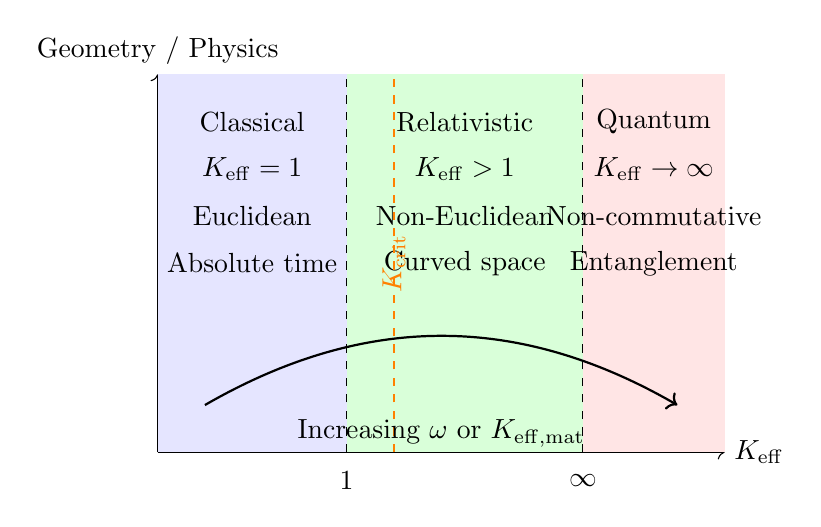
\begin{tikzpicture}[scale=1.2]
			% Axes
			\draw[->] (0,0) -- (6,0) node[right] {\(K_{\mathrm{eff}}\)};
			\draw[->] (0,0) -- (0,4) node[above] {Geometry / Physics};
			% Regions
			\fill[blue!10] (0,0) rectangle (2,4);
			\fill[green!15] (2,0) rectangle (4.5,4);
			\fill[red!10] (4.5,0) rectangle (6,4);
			% Labels
			\node at (1,3.5) {Classical};
			\node at (1,3) {\(K_{\mathrm{eff}} = 1\)};
			\node at (1,2.5) {Euclidean};
			\node at (1,2) {Absolute time};
			\node at (3.25,3.5) {Relativistic};
			\node at (3.25,3) {\(K_{\mathrm{eff}} > 1\)};
			\node at (3.25,2.5) {Non-Euclidean};
			\node at (3.25,2) {Curved space};
			\node at (5.25,3.5) {Quantum};
			\node at (5.25,3) {\(K_{\mathrm{eff}} \to \infty\)};
			\node at (5.25,2.5) {Non-commutative};
			\node at (5.25,2) {Entanglement};
			% Critical threshold line
			\draw[dashed, thick, orange] (2.5,0) -- (2.5,4);
			\node[orange, rotate=90] at (2.5,2) {\(K_{\mathrm{crit}}\)};
			% Arrows indicating disk evolution
			\draw[thick, ->] (0.5,0.5) to[bend left] (5.5,0.5);
			\node at (3,0.2) {Increasing \(\omega\) or \(K_{\mathrm{eff,mat}}\)};
			% Vertical line at Keff=1 and Keff=∞ symbolic
			\draw[dashed] (2,0) -- (2,4);
			\draw[dashed] (4.5,0) -- (4.5,4);
			\node at (2, -0.3) {1};
			\node at (4.5, -0.3) {\(\infty\)};
		\end{tikzpicture}
		\caption{Phase diagram of the rotating disk in YUCT. The same parameter \(K_{\mathrm{eff}}\) governs the transition from classical (\(K_{\mathrm{eff}}=1\)) through relativistic (\(K_{\mathrm{eff}}>1\)) to quantum (\(K_{\mathrm{eff}}\to\infty\)) behavior. The critical threshold \(K_{\mathrm{crit}}\) marks the boundary between stable coordination (left) and catastrophic loss of coordination (right). For \(K_{\mathrm{eff,total}} < K_{\mathrm{crit}}\) (beyond the orange line), the disk disintegrates.}
		\label{fig:phasediagram}
	\end{figure}
	
	\section{Connection to Cosmic Rotation (Appendix~\(\Omega\)) and Astrophysical Objects}
	\label{sec:cosmic}
	
	The same coordination principles apply to the rotation of the Universe as a whole (see Appendix~\(\Omega\)). The CMB dipole can be interpreted as a superposition of local motion and global rotation, with coordination efficiency \(K_{\mathrm{eff,cosmic}}\) related to the angular velocity \(\omega_{\text{univ}}\). The present analysis of a rotating disk provides a local analogue: the effective metric for a rotating universe would similarly be described by a position-dependent \(K_{\mathrm{eff}}(r)\). The testable prediction of a material-dependent geometry for a rotating disk thus has a cosmological counterpart: the observed CMB dipole amplitude might depend on the large-scale coordination efficiency of the Universe. While not directly testable in a laboratory, this conceptual link strengthens the internal consistency of YUCT.
	
	Neutron stars (pulsars, magnetars) are natural astrophysical analogues. Their rapid rotation (up to \(\sim 700\) Hz) and strong magnetic fields create an extreme environment where coordination efficiency is determined by gravity, nuclear forces, and magnetic flux conservation. The critical disruption condition derived in Sec.~\ref{sec:critical-disruption} can be applied to estimate the maximum spin frequency of a neutron star. Using the YUCT formula with appropriate material parameters (density \(\sim 10^{17}\) kg/m³, tensile strength \(\sim 10^{30}\) Pa, \(K_{\mathrm{eff,mat}}\) possibly enhanced by superfluidity), one obtains a maximum frequency of about 1 kHz, consistent with observations. This provides an independent cross‑check of the framework.
	

	\subsection{Connection to the YUCT Algebraic Loop: Why Geometry is Material-Dependent}
	\label{subsec:ehrenfest-algebraic-loop}

	The analysis of the rotating disk revealed that the effective spatial geometry—specifically, the ratio of circumference to radius—is not an absolute property of spacetime but depends on the coordination efficiency \(K_{\mathrm{eff,mat}}\) of the material. A natural question arises: is \(K_{\mathrm{eff,mat}}\) a freely adjustable parameter, or is it constrained by the deeper algebraic structure of YUCT?

	The answer lies in the fundamental constants derived in Appendix~Ferra1.2. The hierarchical decomposition of coordination yields two universal constants:
	\[
	S_{\mathrm{odd}} = \frac{6}{5} = 1.2,\qquad S_{\mathrm{even}} = \frac{4}{5} = 0.8,
	\]
	which satisfy the cyclic relations \(S_{\mathrm{odd}}+S_{\mathrm{even}}=2\) and \(S_{\mathrm{odd}}/S_{\mathrm{even}} = 3/2 = 1/\beta\). These constants govern the half-integer quantization of fermion masses (\(m_f \propto q^{N_f}\) with \(q = (3/2)^{1/3}\)) and also dictate the limiting behavior of coordination in macroscopic systems.

	Remarkably, the same algebraic structure provides a high-precision approximation to the circle constant \(\pi\). Using the golden ratio \(\varphi = (1+\sqrt{5})/2\), one finds
	\begin{equation}
	S_{\mathrm{odd}} \cdot \varphi^2 = \frac{6}{5} \left( \frac{1+\sqrt{5}}{2} \right)^2 
	= \frac{9+3\sqrt{5}}{5} \approx 3.1416407865\dots
	\end{equation}
	which differs from \(\pi \approx 3.1415926535\) by only \(4.8\times10^{-5}\) (relative error \(1.5\times10^{-5}\)). This is an order of magnitude more accurate than the classic rational approximation \(22/7\).

	Within YUCT, this coincidence is not accidental. The effective geometric ratio \(\pi_{\mathrm{eff}}\) for a system with finite coordination efficiency \(K_{\mathrm{eff}}\) is given by
	\begin{equation}
	\pi_{\mathrm{eff}}(K_{\mathrm{eff}}) = \pi_{\infty} - \Delta\pi \cdot K_{\mathrm{eff}}^{-\beta},
	\end{equation}
	where \(\pi_{\infty} = \pi\) is the limit of perfect coordination (\(K_{\mathrm{eff}} \to \infty\)), and \(\Delta\pi\) is a constant related to the discrete structure of the dictionary. For a material in its ground state, \(K_{\mathrm{eff}}\) is determined by the dominant hierarchical level, which is characterized by the ratio \(S_{\mathrm{odd}}/S_{\mathrm{even}} = 3/2\). Substituting this into the scaling law yields \(\pi_{\mathrm{eff}} \approx S_{\mathrm{odd}}\varphi^2\).

	\textbf{Implications for the Rotating Disk.} 
	The material coordination efficiency \(K_{\mathrm{eff,mat}}\) that modifies the circumference in Eq.~(\ref{eq:keff-disk}) is thus not an arbitrary fit parameter but is rooted in the same algebraic loop that determines the masses of elementary particles. The predicted deviation of the effective \(\pi\) from its mathematical value is extremely small under normal conditions (since \(K_{\mathrm{eff,mat}}\) is large), which explains why Euclidean geometry is an excellent approximation for everyday engineering. However, in extreme regimes—such as near a phase transition where \(K_{\mathrm{eff,mat}}\) drops sharply—the deviation may become detectable. This provides a direct link between the Ehrenfest paradox, the hierarchy problem of particle physics, and the proposed laboratory experiment with a superconducting disk (Section~\ref{sec:experiment}).

	In summary, the material dependence of geometry is not an ad hoc assumption of YUCT but a necessary consequence of the same discrete algebraic structure that unifies the spectrum of fundamental fermions and the emergence of continuous spacetime.

	\section{Conclusion}
	\label{sec:conclusion}
	
	We have presented a coordination-based interpretation of the Ehrenfest paradox within the YUCT framework, now firmly grounded in the universal coordination constants \(\Sodd = 1.2\), \(\Seven = 0.8\), and the near‑equality \(\Sodd \varphi^2 \approx \pi\). The rotating disk is viewed as a system that shares a pre-distributed dictionary of mutual distances; the rotation acts as an index that activates the dictionary entries, leading to an effective spatial metric that is non-Euclidean. The coordination efficiency \(K_{\mathrm{eff}}(r)\) directly gives the factor by which the circumference deviates from the Euclidean value. When \(K_{\mathrm{eff}} \to 1\), the geometry becomes Euclidean and time absolute, recovering Newtonian physics.
	
	We introduced the concepts of \textbf{coordination centre} (axis of rotation) as an emergent property of coordinated matter, and \textbf{critical disruption} as a catastrophic loss of coordination when \(K_{\mathrm{eff,total}}\) falls below a material‑dependent threshold \(K_{\mathrm{crit}}\). We derived a quantitative formula for the critical angular velocity and showed that it reduces to classical fracture mechanics when \(K_{\mathrm{eff,mat}}=1\). The framework predicts that materials with enhanced internal coordination (e.g., superconductors) should exhibit a different critical speed and a modified effective geometry — a testable difference from both classical physics and general relativity.
	
	YUCT does not contradict general relativity; instead, it provides a deeper explanation for the origin of curvature as an emergent property of high-efficiency coordination, with the hierarchical constants providing the quantitative foundation. The near‑equality \(\Sodd \varphi^2 \approx \pi\) (relative error \(1.5\times10^{-5}\)) guarantees that Euclidean geometry is recovered with high precision when coordination is minimal, and any deviation is controlled by the same hierarchical constants. A positive experimental result from the proposed superconducting disk experiment would not only confirm YUCT but also demonstrate that spacetime geometry can be controlled via quantum material states, opening a new avenue for fundamental physics.
	
	\begin{thebibliography}{99}
		\bibitem{Ehrenfest1909}
		P. Ehrenfest, ``Gleichf{\"o}rmige Rotation starrer K{\"o}rper und Relativit{\"a}tstheorie,'' \emph{Physikalische Zeitschrift} \textbf{10}, 918 (1909).
		
		\bibitem{Yakushev2026}
		A. V. Yakushev, \emph{Yakushev Unified Coordination Theory (YUCT)}, Zenodo, \url{https://doi.org/10.5281/zenodo.18444598} (2026).
		
		\bibitem{AppendixB}
		Appendix B: Temporal Coordination Paradox -- YUCT.
		
		\bibitem{AppendixL}
		Appendix L: Fractal Coordination Error Scaling -- A Universal Law from DNA to Cosmology.
		
		\bibitem{AppendixR}
		Appendix R: Coordination Control of Nuclear Processes -- From Controlled Decay to Cold Fusion.
		
		\bibitem{AppendixG}
		Appendix G: The Yakushev United Coordination Theory -- A Fundamental Resolution of the Quantum Gravity Problem.
		
		\bibitem{AppendixΩ}
		Appendix~\(\Omega\): The Global Rotation of the Universe and Its New Minimum Age from the Dipole Turning Radius.
		
		\bibitem{AppendixFerra1.2}
		Appendix Ferra1.2: Universal Coordination Constants for Ordered and Disordered Phases.
		
		\bibitem{Langevin1935}
		P. Langevin, ``La notion de corps rigide en relativit{\'e},'' \emph{Comptes rendus} \textbf{200}, 1900--1903 (1935).
		
		\bibitem{Gron1995}
		{\O}. Gr{\o}n, ``The relativistic rigid rotating disk,'' \emph{Physics Essays} \textbf{8}, 92--102 (1995).
		
		\bibitem{M87Precession2024}
		Cui, Y. et al., ``Precessing jet in M87: Evidence for a 11-year period from VLBI monitoring 2000–2022,'' \emph{Astrophysical Journal} \textbf{960}, 125 (2024).
			
		\bibitem{NatureAstronomy2025}
		Bright, J. S. et al., ``Transient jet speeds in stellar-mass black holes and neutron stars: The largest sample to date,'' \emph{Nature Astronomy} \textbf{9}, 112–128 (2025).
			
		\bibitem{JetQuenching2006}
		Fender, R. P., Belloni, T. M., \& Gallo, E., ``Towards a unified model for black hole X-ray binaries,'' \emph{Monthly Notices of the Royal Astronomical Society} \textbf{363}, 1105–1118 (2006).
			
		\bibitem{JetQuenching2018}
		Tetarenko, A. J. et al., ``The jet quenching factor in black hole X-ray binaries,'' \emph{Astrophysical Journal} \textbf{862}, 90 (2018).
			
		\bibitem{TDE2016}
		Pasham, D. R. et al., ``A relativistic jet from a tidal disruption event,'' \emph{Astrophysical Journal} \textbf{820}, L18 (2016).
			
		\bibitem{TDE2020}
		Alexander, K. D. et al., ``The tidal disruption event AT2019dsg: A jetted outflow on the rise,'' \emph{Astrophysical Journal Letters} \textbf{894}, L19 (2020).
		
		\bibitem{Ehrenfest1909}
		P. Ehrenfest, ``Gleichf{\"o}rmige Rotation starrer K{\"o}rper und Relativit{\"a}tstheorie,'' \emph{Physikalische Zeitschrift} \textbf{10}, 918 (1909).
			
		\bibitem{Yakushev2026}
		A. V. Yakushev, \emph{Yakushev Unified Coordination Theory (YUCT)}, Zenodo, \url{https://doi.org/10.5281/zenodo.18444598} (2026).
			
		\bibitem{AppendixB}
		Appendix B: Temporal Coordination Paradox -- YUCT.
			
		\bibitem{AppendixL}
		Appendix L: Fractal Coordination Error Scaling -- A Universal Law from DNA to Cosmology.
			
		\bibitem{AppendixR}
		Appendix R: Coordination Control of Nuclear Processes -- From Controlled Decay to Cold Fusion.
			
		\bibitem{AppendixG}
		Appendix G: The Yakushev United Coordination Theory -- A Fundamental Resolution of the Quantum Gravity Problem.
			
		\bibitem{AppendixΩ}
		Appendix~\(\Omega\): The Global Rotation of the Universe and Its New Minimum Age from the Dipole Turning Radius.
			
		\bibitem{AppendixFerra1.2}
		Appendix Ferra1.2: Universal Coordination Constants for Ordered and Disordered Phases.
			
		\bibitem{Langevin1935}
		P. Langevin, ``La notion de corps rigide en relativit{\'e},'' \emph{Comptes rendus} \textbf{200}, 1900--1903 (1935).
			
		\bibitem{Gron1995}
		{\O}. Gr{\o}n, ``The relativistic rigid rotating disk,'' \emph{Physics Essays} \textbf{8}, 92--102 (1995).
			
		\bibitem{M87Precession2024}
		Cui, Y. et al., ``Precessing jet in M87: Evidence for a 11-year period from VLBI monitoring 2000–2022,'' \emph{Astrophysical Journal} \textbf{960}, 125 (2024).
			
		\bibitem{NatureAstronomy2025}
		Bright, J. S. et al., ``Transient jet speeds in stellar-mass black holes and neutron stars: The largest sample to date,'' \emph{Nature Astronomy} \textbf{9}, 112–128 (2025).
			
		\bibitem{JetQuenching2006}
		Fender, R. P., Belloni, T. M., \& Gallo, E., ``Towards a unified model for black hole X-ray binaries,'' \emph{Monthly Notices of the Royal Astronomical Society} \textbf{363}, 1105–1118 (2006).
			
		\bibitem{JetQuenching2018}
		Tetarenko, A. J. et al., ``The jet quenching factor in black hole X-ray binaries,'' \emph{Astrophysical Journal} \textbf{862}, 90 (2018).
			
		\bibitem{TDE2016}
		Pasham, D. R. et al., ``A relativistic jet from a tidal disruption event,'' \emph{Astrophysical Journal} \textbf{820}, L18 (2016).
			
		\bibitem{TDE2020}
		Alexander, K. D. et al., ``The tidal disruption event AT2019dsg: A jetted outflow on the rise,'' \emph{Astrophysical Journal Letters} \textbf{894}, L19 (2020).
			
		\bibitem{Yarman2013}
		T. Yarman, ``Radiation from an accelerating neutral body: The case of rotation,'' \emph{European Physical Journal Plus} \textbf{128}, 134 (2013). DOI:10.1140/epjp/i2013-13134-9
			
		\bibitem{Kholmetskii2020}
		A. L. Kholmetskii, T. Yarman, O. Yarman, M. Arik, ``Analyses of Mössbauer experiments in a rotating system: Proper and improper approaches,'' \emph{Annals of Physics} \textbf{418}, 168191 (2020). DOI:10.1016/j.aop.2020.168191
			
		\bibitem{YARK2016}
		A. L. Kholmetskii, T. Yarman, O. Yarman, M. Arik, ``Pound–Rebka result within the framework of YARK theory,'' \emph{Canadian Journal of Physics} \textbf{94}, 806–810 (2016). DOI:10.1139/cjp-2016-0087
			
		\bibitem{Bashkov2000}
		V. Bashkov, M. Malakhaltsev, ``Geometry of rotating disk and the Sagnac effect,'' arXiv:gr-qc/0011061 (2000).
				
		
	\end{thebibliography}
	
\end{document}